
\section{Grasping \& Manipulation System}
\label{sec:manip}
%
In this section we present an integrative approach for grasp representation/planning and motion
generation. The main idea is to provide a functional representation of grasps as intervals in task
space, which allows redundancy in the gripper pose prior to executing the grasp. Subsequently, we
leverage the obtained redundancy to generate reactive manipulator motions by formulating a
representation of the corresponding tasks as a hierarchical Stack of Tasks (SoT) which is executed
by the prioritized motion control framework proposed by Kanoun et al.~\cite{Kano11}.
%
\subsection{Challenges in Autonomous Grasping}
\label{subsec:Grasping_challenges}
%
In current autonomous grasping systems~\cite{Bere07, Srin10, Krug14a}, grasp planning and
manipulator motion planning are usually seen as independent sub-problems. A database storing object
models together with sets of pre-computed grasps is used to find suitable gripper poses and joint
configurations. In the online stage, sampling based planners~\cite{LaVa06} attempt to generate valid
trajectories for the pre-planned grasps, which are executed in a feasible-first
manner~\cite{Bere07}. During the execution phase, such approaches necessitate many futile motion
planning attempts, which often incurs significant time delays since sampling based planners suffer
from the curse of dimensionality. Also, while being able to solve complicated planning problems if
given enough time, these planners do not scale well to geometrically simple scenarios and they are
ill suited to incorporate contact events with the environment which is a prerequisite for any
grasping/manipulation application.

Using control to exploit manipulator redundancy has long been in the focus of research~\cite{Sici91,
  Sent10}. In this line of thought, opposed to define a set of discrete grasp poses, Gienger et
al.~\cite{Gien08a, Gien08b} learn a manifold of feasible grasps for an object and use an
attractor-based control scheme to reach the corresponding volume in the task space. Another approach
to address motion planning and motion control simultaneously, is to formulate a hierarchical stack
of equality tasks which are represented as task functions~\cite{Sams91}. Lower-ranked tasks are then
solved in the null-space of tasks with higher priority~\cite{Sici91, Sent10}. A major step forward
in this direction was achieved by Kanoun et al.~\cite{Kano11}, who extended the approach to include
inequality tasks which significantly increases the expressiveness of the method. Recent advancements
include the extension to dynamic control~\cite{Saab13} and an efficient solution algorithm for the
underlying optimization problem~\cite{Esca14}.
%
\subsection{Object Detection}
\label{subsec:obj_det}
%
%
\begin{algorithm}[t!]
%\DontPrintSemicolon
\SetKwInOut{Input}{input}
\SetKwInOut{Output}{output}
\Input{Pointcloud $\mathcal{P}$, transform from sensor frame to world frame $^w_s\mbm{T}(\mbm{q})$}
\Output{Target clusters $\{\mathcal{T}\}$}
Transform $\mathcal{P}$ into world coordinates using $^w_s\mbm{T}(\mbm{q})$\;
\While {target plane not found} {
    Extract pallet plane normal $\mbm{n}$, offset $d$ from $\mathcal{P}$ using RANSAC\;
    \eIf{$\left(\mbm{n}^T\mbm{e}_z < \cos{\alpha}\right) \wedge \left(\text{abs}(d-h_p) < \epsilon_p\right)$}{target
      plane found\;}
     {$\mathcal{P} \leftarrow$ remove inliers\; \If{ $|\mathcal{P}|$ less than $20\%$ of the
        original}{report failure\; \Return\;}}
}
$\mathcal{B} \leftarrow$ oriented bounding box of plane inliers with $z$-component in $(d,d+\epsilon_d)$\;
$\{\mathcal{E}\} \leftarrow$ euclidean cluster points in $\mathcal{B}$\;
\For{each cluster $\mathcal{E}_i$} {
    Fit a ML Gaussian to $\mathcal{E}_i$ as $\mbm{\mu}_i,\mbm{\Sigma}_i$\;
    Eigen decomposition $\mbm{\Sigma_i}=\mbm{Q}\mbm{\Lambda}\mbm{Q}^{-1}$\;
    $\mbm{v}_1 \leftarrow$ eigenvector associated to the largest eigenvalue $\lambda_1$\;
    \If{$(\mbm{v}_1^T\mbm{e}_z < \cos{\epsilon_{\alpha}}) \wedge (\lambda_2 < r_{max})$} {append cluster
      $\mathcal{E}_i$ to the solution set $\{\mathcal{T}\}
      \leftarrow \mathcal{E}_i$\;}
}
\caption{Object detection algorithm}\label{alg:obj}
\end{algorithm}
%
A typical commissioning scenario in a warehouse environment generally involves as a first step the
identification and localization of an object targeted for picking. There are however many
application scenario specific factors to consider when designing an object detection system for this
task. For example: a single pallet may hold a homogeneous or a heterogeneous set of objects; objects
may be stored in boxes and be equipped with barcodes; objects may be stored on shelves, pallets, or
simply be piled up. In this work, we assume a simple scenario where objects of the same type are
stored on a single pallet. As shown in Fig.~\ref{fig:robot}, the gripper of the APPLE system is
equipped with a Structure IO structured light depth sensor\footnote{\url{http://structure.io/}}. We
use the 3D point clouds generated by this sensor as an input for a simple object detection module
which identifies clusters of points matching our expected object models. The object detection module
was implemented using the Point Cloud Library (PCL)~\cite{Rusu11} following the simple procedure
summarized in Algorithm~\ref{alg:obj}.

The basic idea of Algorithm~\ref{alg:obj} is to first detect the location of the pallet plane, then
to extract the points belonging to objects on the pallet, cluster them and subsequently analyze the
obtained clusters. The parameters in this algorithm are the expected height $h_p$ of the
pallet above floor level, a tolerance $\epsilon_p$ on the pallet height, a tolerance
$\epsilon_{\alpha}$ on the angle that the pallet plane normal makes with the vertical axis $\mbm{z}$
and the maximum radius $r_{max}$ of a graspable cylinder. Each of the detected clusters is analyzed
using PCA, checking that the dominant point distribution is along the $\mbm{z}$ axis and that the
$x/y$ point spread is within the graspable objects limit. Identified target clusters are then passed
on to the grasp planning module described below.
%
\subsection{Grasp Representation and Planning}
\label{subsec:grasp_planning}
%
\begin{figure}[t!] 
   \centering
    \def\svgwidth{235pt} 
    \input{figs/grasp_interval.pdf_tex} 
    \caption{\textit{Grasp interval:} The shaded cyan regions illustrate the side grasp interval
      constraints for a cylindrical object. For a successful grasp, the palm frame origin $\mbm{o}$
      needs to lie inside the depicted cylindrical shell which is aligned with object axis
      $\mbm{a}$. The cylinders height is limited by two planes which are normal to
      $\mbm{a}$. Additionally, the gripper's vertical axis ($z$) is constrained to lie in a cone
      whose axis $\hat{\mbm{a}}$ is parallel to the object axis $\mbm{a}$. Furthermore, the
      gripper's approach axis ($x$) has to lie inside a cone centered on the normal which connects
      axis $\mbm{a}$ and point $\mbm{o}$.}
   \label{fig:grasp_interval}
   \vspace{-0.5cm}
\end{figure}
%
Traditional data-driven grasp synthesis~\cite{Bohg14} relies on precise knowledge of the target
object geometry and frictional properties. Since this information is often not available in
practice, grasps planned in simulation might fail. This holds especially true, when considering an
underactuated grasping device as we do in the presented work. In this case, the gripper's joint
configuration depends on the interaction with the environment and is difficult or impossible to
determine at planning time. Instead, we represent grasps as pre-defined pose intervals associated
with primitive object geometries as exemplary shown in Fig.~\ref{fig:grasp_interval} for side grasps
on cylindrical objects. Note that an analogue interval can also be formed to enable top
grasps. These intervals bound the grasping device's position and orientation, but do not fully
constrain its pose. In this work, for simplicity, we limit ourselves to the illustrated grasp
interval defined for cylindrical shapes. Corresponding intervals can be defined for other shape
categories such as spheres and parallelepipeds as well. Opposed to the similarly defined task
intervals in~\cite{Gien08a, Gien08b} which are learned in simulation, we deliberately design grasp
intervals to incorporate prior knowledge about robust grasp poses in our representation. In a
concept originating from observations of human grasping behavior, it has been shown that the
grasping device should be roughly aligned with the target object's principal components to achieve
robust grasps~\cite{Bala12}. This property is achieved by the cone constraints for the case depicted
in Fig.~\ref{fig:grasp_interval}.

Currently, the parameters of the grasp intervals such as the distance range between gripper and
object have to be evaluated experimentally for each primitive shape category. To ease this
non-trivial requirement, in the presented work we rely on a gripper which offers a low pre-grasp
pose sensitivity combined with a compliant and robust grasp execution routine as discussed in
Section~\ref{subsec:grasp_execution}.
%
\begin{figure}[t!] 
   \centering
    \def\svgwidth{235pt} 
    \input{figs/truncated_grasp_interval.pdf_tex} 
    \caption{\textit{Truncated grasp interval:} During the online stage, the corresponding grasp
      interval shown in Fig.~\ref{fig:grasp_interval} needs to be truncated ($i.\,e.,$ parameters
      for $r_1$, $r_2$, $c$, $h$ and $\varphi$ need to be determined) to accommodate the specific
      target object dimensions and to account for the fact that some regions of the grasp interval
      might not be feasible due to obstruction by the environment.}
   \label{fig:truncated_grasp_interval}
   \vspace{-0.5cm}
\end{figure}

During operation, after the target object pose is detected as the mean and covariance of the cluster
obtained from Algorithm~\ref{alg:obj}, the grasp interval needs to be adapted to the specific scene
and target object dimensions as illustrated in Fig.~\ref{fig:truncated_grasp_interval}. For the
evaluation presented in Section~\ref{sec:eval} we pre-defined the corresponding parameters and
gripper pre-grasp joint configuration, an appropriate programmatic approach is left to future work.
One promising strategy currently being explored is to pre-compute a gripper collision map and use it
for determining the valid grasping configurations around the target object. Once invalid grasping
configurations have been pruned by using the scene model, the remaining configurations can be
clustered into continuous regions and used to determine the constraints in an automatic and
collision-aware manner.
%
\subsection{Manipulator Motion Generation}
\label{subsec:manip_motion}
%
To leverage the freedom in pre-grasp position and orientation gained from the previously described
grasp representation, we use a control-based approach for reactive, on-the-fly motion
generation. More specific, the method of choice is the one developed by Kanoun et al.~\cite{Kano11}
which allows to formulate the grasp interval, as well as additional desiderata such as joint limit
avoidance, in form of task functions which subsequently are utilized to form a hierarchical SoT. In
this paradigm, the SoT is then used to compute prioritized controls during movement
execution. Therefore, motions are generated instantaneously without the planning delays occurring in
sense-plan-act architectures. In the following, we briefly revise the concept. For an in-depth
discussion the reader is referred to the original work presented in~\cite{Kano11}.

We lean on the notation in~\cite{Esca14} and define the manipulator joint configuration by the
vector $\mbm{q}$ and the control inputs as corresponding joint velocities $\dot{\mbm{q}}$. A task
function is any derivable function of $\mbm{q}$. To give an example, a task with the purpose of
bringing an end-effector point $\mbm{p}(\mbm{q})$ onto a plane described by unit normal $\mbm{n}$
and offset $d$ can be transcribed by the task function $\mbm{e}=\mbm{n}^T\mbm{p}(\mbm{q})-d$, which
formulates the projection residual between the plane and $\mbm{p}(\mbm{q})$. The task evolution is
given by $\mbm{J}\dot{\mbm{q}}=\dot{\mbm{e}}$ with task jacobian
$\mbm{J}=\frac{\partial\mbm{e}}{\partial\mbm{q}}$.

The goal is to compute joint velocities such that the task evolution follows a desired reference
profile $\dot{\mbm{e}}^*$ (in this work chosen as exponential decay $\dot{\mbm{e}}^*= -\lambda
\mbm{e}$, with $\lambda \in \mathbb{R}_+$). For a single equality task, this necessitates to solve
the following least squares Quadratic Program (QP)
%
\begin{align}\label{eq:QP}
  \dot{\mbm{q}}^* &\in \mbox{arg} \; \underset{\footnotesize\dot{\mbm{q}}\normalsize}{\mbox{min}}||\mbm{J}\dot{\mbm{q}}-\dot{\mbm{e}}^*||.
\end{align}
%
In order to allow for inequality tasks, we henceforth use a general task formulation with upper
bounds 
\begin{align}\label{eq:task}
  \mbm{J}\dot{\mbm{q}}&\leq \dot{\mbm{e}}^*.
\end{align}
%
As stated in~\cite{Esca14}, this allows to transcribe lower bounds \mbox{$\mbm{J}\dot{\mbm{q}} \geq
  \dot{\mbm{e}}^*$,} double bounds \mbox{$\dot{\underline{\mbm{e}}}^* \leq \mbm{J}\dot{\mbm{q}} \leq
  \dot{\bar{\mbm{e}}}^*$} and equalities \mbox{$\mbm{J}\dot{\mbm{q}}=\dot{\mbm{e}}^*$} by
reformulating the task respectively as
\mbox{$-\mbm{J}\dot{\mbm{q}} \leq -\dot{\mbm{e}}^*$,} $\begin{bmatrix} -\mbm{J} \\
  \mbm{J} \end{bmatrix}\dot{\mbm{q}} \leq \begin{bmatrix} -\dot{\underline{\mbm{e}}}^*
  \\ \dot{\bar{\mbm{e}}}^* \end{bmatrix}$ and $\begin{bmatrix} -\mbm{J} \\
  \mbm{J} \end{bmatrix}\dot{\mbm{q}} \leq \begin{bmatrix} -\dot{\mbm{e}}^* \\
  \dot{\mbm{e}}^* \end{bmatrix}$.

If the constraint in~\eqref{eq:task} is infeasible, a least squares solution for $\dot{\mbm{q}}^*$ as
in~\eqref{eq:QP} can be found by introducing the slack variable $\mbm{w}$ in the decision variables
%
\begin{align}\label{eq:iQP}
  &\underset{\dot{\mbm{q}},\;\mbm{w}}{\mbox{min}}\;\;||\mbm{w}||\\
   \mbox{subject to} \quad &\mbm{J}\dot{\mbm{q}} \leq \dot{\mbm{e}}^* + \mbm{w}. \nonumber
\end{align}
%
To form a hierarchical SoT with $p=1,\dots,P$ priority levels, we stack all task jacobians
in~\eqref{eq:task} with the same assigned priority in a matrix $\mbm{A}_p$, and all corresponding
reference velocities in a vector $\mbm{b}_p$ to form one constraint of the form
$\mbm{A}_p\dot{\mbm{q}}\leq \mbm{b}_p$ for each hierarchy level. The aim is to sequentially satisfy
a constraint at best in the least square sense while solving for the subsequent constraint of lower
priority in the null-space of the previous constraint, such that the previous solution is left
unchanged. Therefore, the following QP, where the previous slack variable solutions $\mbm{w}_i^*$
are frozen between iterations, needs to be solved for $p=1,\ldots,P$
%
\begin{align}\label{eq:HiQP}
  &\underset{\dot{\mbm{q}},\;\mbm{w}_p}{\mbox{min}}\;\;||\mbm{w}_p||\\
   \mbox{subject to} \quad &\mbm{A}_i\dot{\mbm{q}} \leq \mbm{b}_i + \mbm{w}_i^*, \quad i=1,\dots,p-1 \nonumber \\
                           &\mbm{A}_p\dot{\mbm{q}} \leq \mbm{b}_p + \mbm{w}_p.  \nonumber 
\end{align}
%
The final control vector $\dot{\mbm{q}}^*$ is then obtained from the $P^{\mbox{th}}$ solution
of~\eqref{eq:HiQP}. Opposed to sampling based planners, the chosen control scheme allows to
incorporate qualitative requirements ($e.\,g.$, the desired gripper alignment) during motion
generation and allows for redundancy exploitation via appropriate task function formulations.

Manipulator obstacle avoidance is also achieved on a control level, by formulating tasks which
maintain minimum distances between simple geometric primitives such as spheres, planes, points and
capsules. We argue that for the considered application strict collision avoidance is neither
necessary nor desired, since picking and manipulation inherently necessitates contact events between
the robot and the environment. Also, in real-world applications where knowledge about the
environment is available only in form of noisy sensor data, it might not be possible to avoid
contact with the environment without being overly conservative. To this end, the APPLE platform
relies on the compliant low-level control schemes and contact detection abilities of the employed
manipulator.
%
\subsection{Robust Grasp Execution}
\label{subsec:grasp_execution}
%
\begin{figure}[!t]
 \centering
   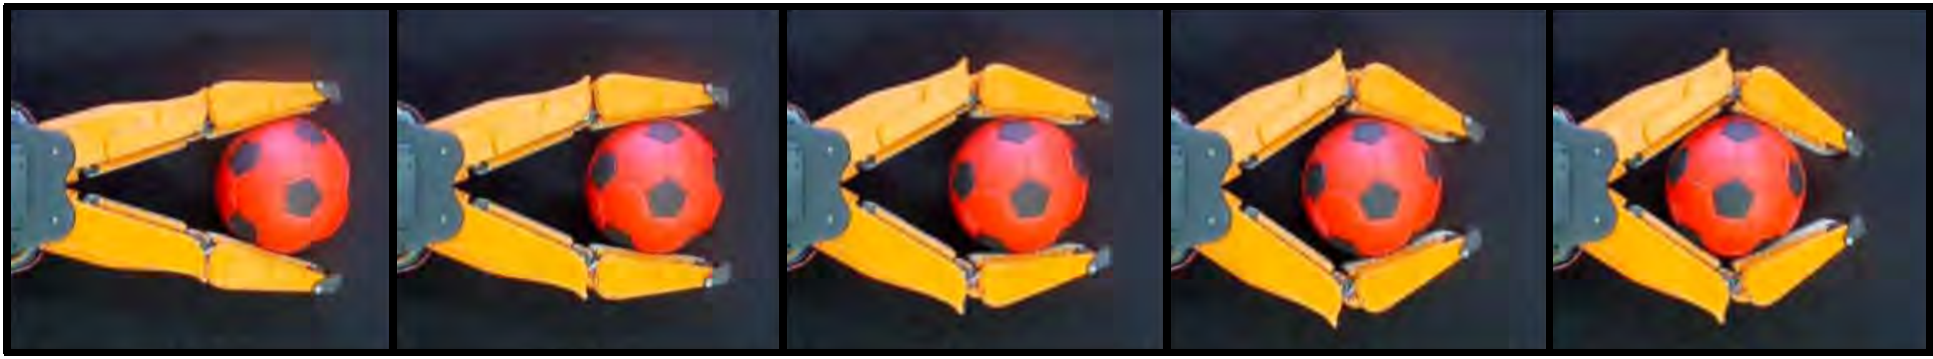
\includegraphics[width = 1.0\linewidth]{figs/pull_in}
   \caption{\textit{Pull-in grasping strategy:} Depicted is a sequence of intermediate grasp states
     where the belts of the gripper are used to pull the object towards its palm which results in a
     transition from a fingertip to an enveloping grasp.}
   \vspace{-4mm}
   \label{fig:pull_in}
   \centering
 \end{figure}
 % 
 \begin{figure*}[!t]
   \centering
   \subfigure[]{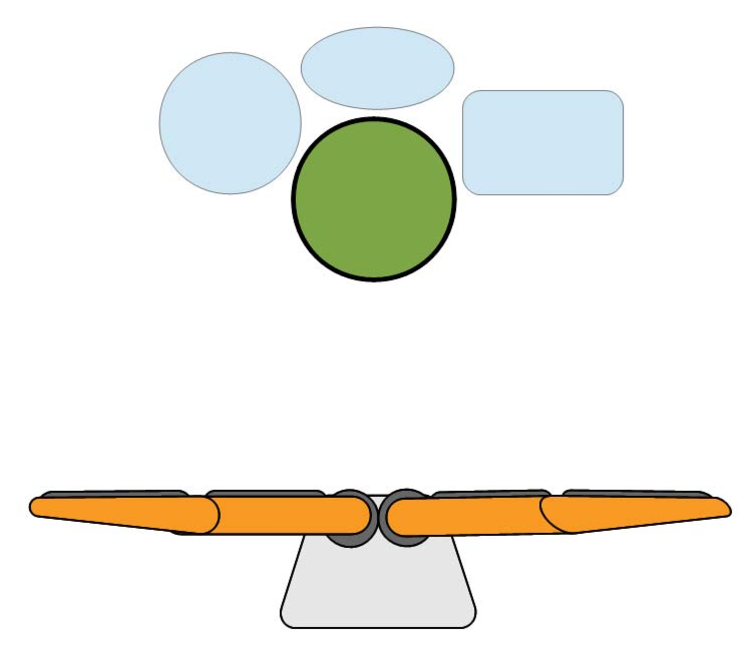
\includegraphics[width = .32\linewidth]{figs/vcg1}}
   \subfigure[]{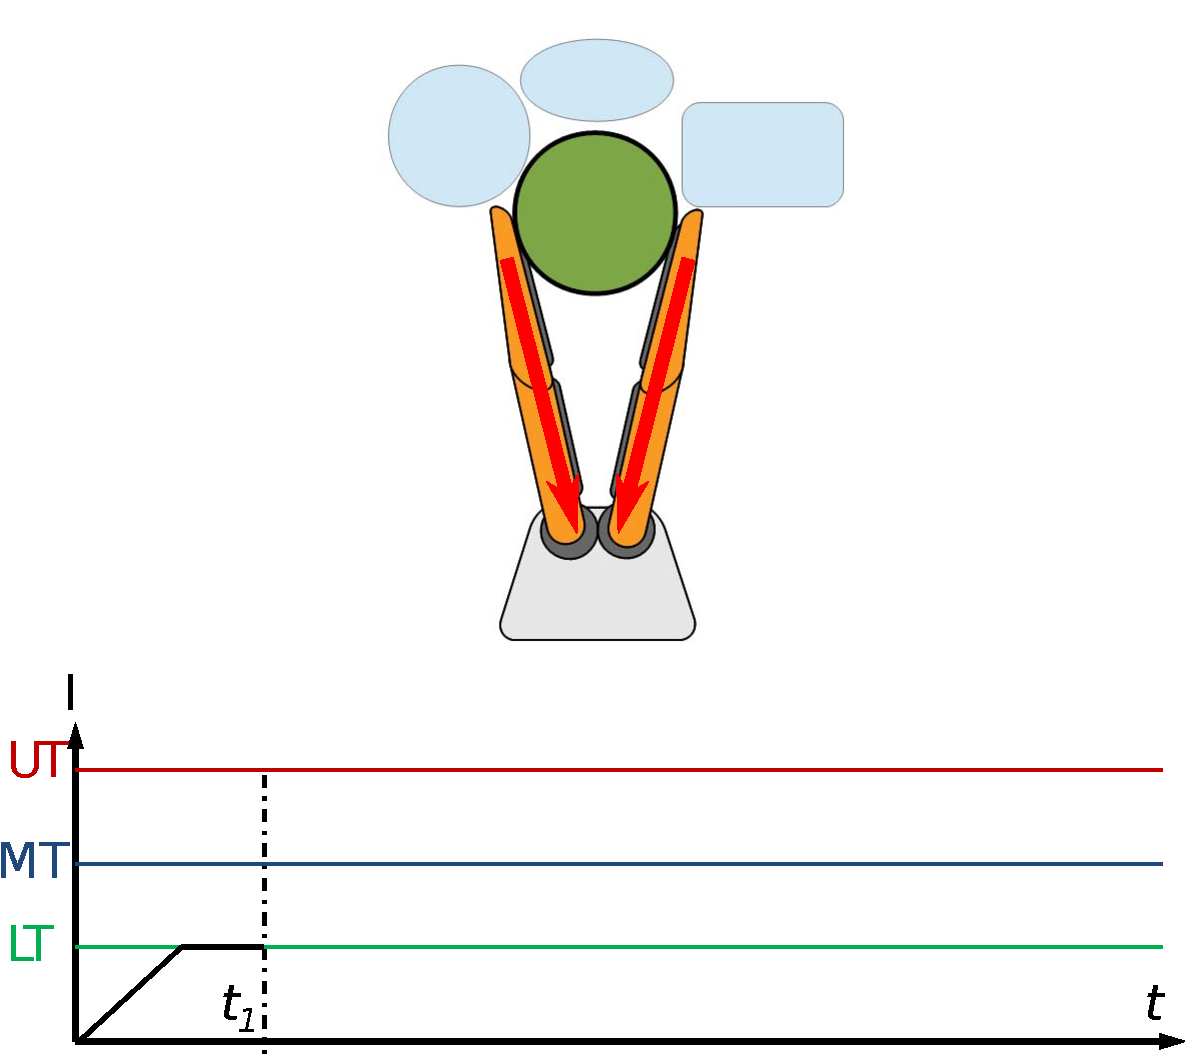
\includegraphics[width = .32\linewidth]{figs/vcg2}}
   \subfigure[]{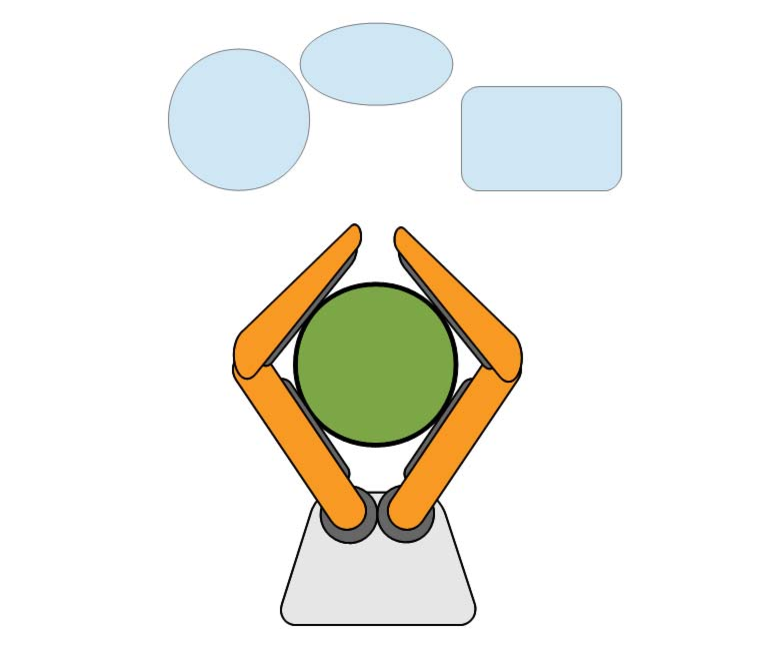
\includegraphics[width = .32\linewidth]{figs/vcg3}}
   \caption{\textit{Grasp Execution Control:} (Left) as the gripper starts closing, the current
     through the opening motor is monitored; (Middle) when contact is made, the actuated belts are
     switched on to pull in the object; (Right) the controller strives to maintain a given current
     setpoint to enable compliant in-hand manipulation behavior;}
   \label{fig:pull_in_control}
   \centering
   \vspace{-0.5cm}
 \end{figure*}
%
 For this component, we exploit the capabilities of the utilized gripper~\cite{Tinc12}, namely
 underactuation and conveyor belts on the finger pads in order to achieve robust grasping
 behavior. Each of the gripper’s two fingers has a planar manipulator structure with two rotary
 joints and active surfaces which are implemented by conveyor belts on the inside of the two
 phalanges. The mechanical structure is underactuated and comprises only one actuated Degree of
 Freedom (DoF) for opening and closing and two DoF per finger for the belt movements. If, during
 grasping, the proximal phalanges are blocked by an object, the gripper’s distal phalanges continue
 to ``wrap around'' and envelope it in a firm grasp. The experiments reported in~\cite{Krug14a}
 showed, that in cluttered scenes fingertip grasps are more likely to be feasible than robust
 enveloping grasps, because the latter necessitate large opening angles resulting in bulky gripper
 silhouettes for which there might no collision free approach trajectory exist. Therefore, we employ
 the ``pull-in'' strategy which is illustrated in Fig.~\ref{fig:pull_in}. As demonstrated
 previously~\cite{Krug14c}, this strategy is especially effective in achieving stable grasps,
 starting from a relatively wide range of initial gripper poses with respect to the target object.
\par
The grasping controller was implemented by means of low-level current control of the gripper's
actuators. Since the gripper drives have a low transmission ratio and are easily back-driveable,
current control enables a simple compliant behavior because the current absorption increases with
increasing effort on the output. Thus, in the present case, the motor current is proportional to the
resulting grasping force. The developed grasping strategy is implemented in three steps as
illustrated in Fig.~\ref{fig:pull_in_control}. First, a relatively low current setpoint is given to
the open/close motor controller and the fingers start closing. Once the fingers come into contact
with the object and the target current is reached, the motion stops which is detected by monitoring
the corresponding motor encoder. Now the second phase of the grasping process is triggered and the
belts are actuated to pull in the target object.  We then monitor the encoders on the belts and on
the phalange joints. If the belts block and the phalanges have wrapped around the object, an
enveloping grasp is achieved and we transition to the final stage. Here, a higher current setpoint
is given to the open/close motor controller to ensure a firm grasp. The main parameters to this
routine (the current thresholds for contact and final enveloping grasp) depend on the target object
properties -- namely friction coefficient and mass. In this work, the parameters were
experimentally tuned and good values were found for a set of common household objects.
